\documentclass[english]{textolivre}

% metadata
\journalname{Texto Livre}
\thevolume{18}
%\thenumber{1} % old template
\theyear{2025}
\receiveddate{\DTMdisplaydate{2024}{7}{31}{-1}}
\accepteddate{\DTMdisplaydate{2024}{11}{29}{-1}}
\publisheddate{\DTMdisplaydate{2025}{4}{17}{-1}}
\corrauthor{Pablo Ramírez Rodríguez}
\articledoi{10.1590/1983-3652.2025.53794}
%\articleid{NNNN} % if the article ID is not the last 5 numbers of its DOI, provide it using \articleid{} commmand 
% list of available sesscions in the journal: articles, dossier, reports, essays, reviews, interviews, editorial
\articlesessionname{dossier}
\runningauthor{Ramírez Rodríguez y Antonov}
%\editorname{Leonardo Araújo} % old template
\sectioneditorname{Hugo Heredia Ponce}
\layouteditorname{João Mesquita}

\title{New challenges and opportunities in technology-assisted phraseology interpreting: the case of Yandex live stream translation}
\othertitle{Novos desafios e oportunidades na interpretação da fraseologia assistida pela tecnologia: o caso da tradução de vídeo ao vivo do Yandex}
%\othertitle{Nuevos retos y oportunidades en la interpretación de la fraseología asistida por la tecnología: el caso de la traducción de vídeo en directo de Yandex}

\author[1]{Pablo Ramírez Rodríguez~\orcid{0000-0002-6168-3736}\thanks{Email: \href{mailto:pablorarod@gmail.com}{pablorarod@gmail.com}}}
\author[2]{Evgeniy Antonov~\orcid{0000-0003-1498-9131}\thanks{Email: \href{mailto:eantonov@kaf65.ru}{eantonov@kaf65.ru}}}
\affil[1]{Universidad de Granada, Granada, Spain.}
\affil[2]{National Research Nuclear University, MEPhI, Moscow, Russia.}

\addbibresource{article.bib}
%\usepackage{easyReview}
% \usepackage[utf8]{inputenc}  % UTF-8 encoding for Unicode characters
% \usepackage[T2A]{fontenc}    % Cyrillic font encoding for Russian characters

\setotherlanguage{russian}   % Define another language
%\usepackage{fontspec}      % For font selection
%\newfontfamily\cyrillicfont[Script=Cyrillic]{Charis SIL}
%\newfontfamily\cyrillicfont{Liberation Serif}
\newfontfamily\cyrillicfontsf{Liberation Sans}

\begin{document}
\maketitle
\begin{polyabstract}
%\begin{spanish}
%\begin{abstract}
%  La interpretación asistida por ordenador (IAO) se ha convertido
%  en un elemento esencial en un mundo cada vez más globalizado e
%  interconectado. Con la creciente demanda de comunicación instantánea en
%  línea y la necesidad de superar las limitaciones lingüísticas en un
%  contexto global, la IAO se ha convertido en una valiosa herramienta para
%  una amplia gama de aplicaciones. Sin embargo, la IAO no está exenta de
%  dificultades. La interpretación de expresiones idiomáticas sigue siendo
%  un obstáculo importante, ya que estas construcciones lingüísticas pueden
%  ser especialmente difíciles de interpretar con precisión debido a su
%  naturaleza culturalmente arraigada. En este contexto, el objetivo de
%  este artículo es abordar el problema de la interpretación de expresiones
%  idiomáticas, en nuestro caso de 52 locuciones verbales en el marco de la
%  IAO, centrándonos en la combinación lingüística español-ruso. El
%  objetivo es analizar cómo esta tecnología responde a los retos de la
%  fraseología idiomática y cómo influye en una comunicación intercultural
%  precisa y eficaz. Para lograr este objetivo, se ha aplicado una
%  metodología exhaustiva que combina el análisis lingüístico con
%  observaciones prácticas de situaciones de interpretación asistida por
%  tecnología en tiempo real utilizando el traductor de voz en directo y
%  los contenidos multimedia proporcionados por Yandex. Los resultados de
%  esta investigación aportan una comprensión más profunda de cómo la
%  tecnología de la traducción y la interpretación aborda los retos de la
%  expresión idiomática, al tiempo que proporcionan una visión crítica de
%  la eficacia y las limitaciones de las soluciones tecnológicas en el
%  ámbito de la comunicación intercultural.
%  
%
%
%\keywords{IAO \sep Fraseología \sep Locuciones verbales \sep Traducción en
%directo \sep Interpretación automática}
%\end{abstract}
%\end{spanish}

\begin{english}
\begin{abstract}
Computer-assisted interpreting (CAI) has become an essential
element in an increasingly globalized and interconnected world. With the
growing demand for instant online communication and the need to overcome
language limitations in a global context, CAI has become a valuable tool
for a wide range of applications. However, the CAI is not without its
challenges. The interpretation of idiomatic expressions remains a
significant barrier, as these linguistic constructs can be particularly
difficult to interpret accurately due to their culturally embedded
nature. In this context, the objective of this article is to address the
problem of interpreting idiomatic expressions, in our case 52 verbal
idioms within the framework of CAI, focusing on the Spanish-Russian
language combination. The aim is to analyze how this technology meets
the challenges of idiomatic phraseology and how it influences accurate
and effective intercultural communication. To achieve this goal, a
comprehensive methodology has been applied, combining linguistic
analysis with practical observations of real-time technology-assisted
interpreting situations using the live on-air speech translator and
multimedia content provided by Yandex. The results of this research
provide a deeper understanding of how translation and interpreting
technology addresses the challenges of idiomatic expression, while also
providing critical insight into the effectiveness and limitations of
technological solutions in the field of intercultural communication.

\keywords{CAI \sep Phraseology \sep Verbal idioms \sep Live stream translation \sep
Automatic interpreting} 
\end{abstract}
\end{english}

\begin{portuguese}
\begin{abstract}
  A interpretação assistida por computador (IAC) tornou-se um
  elemento essencial em um mundo cada vez mais globalizado e
  interconectado. Com a crescente demanda por comunicação instantânea
  online e a necessidade de superar as limitações linguísticas em um
  contexto global, a IAC se tornou uma ferramenta valiosa para uma ampla
  gama de aplicações. No entanto, a IAC não está isenta de dificuldades. A
  interpretação de expressões idiomáticas continua sendo um obstáculo
  significativo, pois essas construções linguísticas podem ser
  especialmente difíceis de interpretar com precisão devido à sua natureza
  culturalmente enraizada. Nesse contexto, o objetivo deste artigo é
  abordar o problema da interpretação de expressões idiomáticas, no nosso
  caso de 52 locuções verbais no âmbito da IAC, focando na combinação
  linguística espanhol-russo. O objetivo é analisar como essa tecnologia
  responde aos desafios da fraseologia idiomática e como influencia uma
  comunicação intercultural precisa e eficaz. Para alcançar esse objetivo,
  foi aplicada uma metodologia exaustiva que combina a análise linguística
  com observações práticas de situações de interpretação assistida por
  tecnologia em tempo real, utilizando o tradutor de voz ao vivo e os
  conteúdos multimídia fornecidos pela Yandex. Os resultados desta
  pesquisa proporcionam uma compreensão mais profunda de como a tecnologia
  de tradução e interpretação enfrenta os desafios da expressão
  idiomática, ao mesmo tempo que oferecem uma visão crítica da eficácia e
  das limitações das soluções tecnológicas no âmbito da comunicação
  intercultural.
  
\keywords{IAC \sep Fraseologia \sep Locuções verbais \sep Tradução em tempo
real \sep Interpretação automática}
\end{abstract}
\end{portuguese}


\end{polyabstract}

\section{Introduction}\label{sec-intro}

Technology-assisted interpreting has experienced exponential growth in
recent years, reflected in the dizzying progress in the development of
information and communication technology (ICT) tools and resources
\cite{gutierrezArtacho2016,mezcua2019}. These innovative
technologies have greatly facilitated the interpretation and
comprehension of texts in different linguistic contexts \cite{olallaSoler2015}. In this sense, computer-assisted interpreting (CAI)
has become crucial in an increasingly globalised and connected society,
playing a pivotal role in breaking down language barriers and
facilitating effective communication in an environment characterised by
cultural and linguistic diversity \cite{mellinger2019,li2021}. In
response to the growing demand for instant online communication and the
need to overcome language limitations in a global environment, CAI has
established itself as an infallible tool for a wide range of
applications, from interpreting international business meetings to
translating multimedia content in real time \cite{fantinuoli2017a,alcaidemartinez2021}.

The integration of technology has revolutionised the way individuals
interact with language, opening new possibilities for increasing the
efficiency and accuracy of text interpretation, both in real time and
asynchronously \cite{gaber2023a,ramirezRodriguez2023}. The development
of ICT tools has led to improvements in natural language processing,
machine translation, speech recognition and other related technologies,
resulting in significant advances in text interpretation \cite{valeroGarces2024}. These tools have been particularly useful in overcoming language
barriers in multicultural environments, facilitating communication
between speakers of different languages and promoting intercultural
understanding \cite{perez2020}.

The use of CAI does, however, present certain difficulties. In the
phraseological domain, understanding idiomatic expressions remains a
significant challenge, as these linguistic constructions can be
particularly difficult to interpret accurately due to their cultural
embeddedness \cite{corpaspastorgaber2021,ramirezRodriguez2022}.
Cultural and contextual differences can lead to inaccurate or ambiguous
translations of these expressions, resulting in misunderstandings and
communication problems. In addition, CAI is often based on pre-defined
algorithms and databases, which can limit its ability to adapt to new
idioms and emerging expressions \cite{ortigoza2024}. This problem
identified in the interpretation of idiomatic expressions by CAI adds to
the previously mentioned challenges in technology-assisted phraseology,
where accuracy and fluency in the interpretation of texts in different
linguistic contexts are key to effective communication. The complexity
of idiomatic expressions, such as idioms, and their culturally
contextual nature require new approaches and specialised tools to
improve the interpretation of such expressions, which represents a
relevant area of research in the development of technology-assisted
phraseology.
\section{Theoretical Framework}\label{sec-theoretical}
\subsection{The phraseology-technology binomial}\label{sub-sec-thephraseologytechnology}

Today, phraseology and technology have significantly converged with the
advent of the internet and social networks \cite{corpas2013}.
Phraseology constitutes a specialized field of linguistic study that
focuses on fixed or semi-fixed expressions within a language,
encompassing idiomatic expressions, collocations, and other multi-word
units. Idiomatic expressions are characterized by meanings that cannot
be directly inferred from the literal interpretation of their
constituent elements, as their comprehension relies heavily on cultural
and contextual factors. These expressions pose significant challenges in
interpretation and translation due to their language-specific,
figurative nature and nuanced usage. Thus, phraseology systematically
explores the structural, semantic, and functional dimensions of these
expressions, emphasizing their linguistic and cultural specificity.

In parallel, within the realm of technology, the concept of CAI pertains
to the application of technological tools and specialized software to
augment the interpreting process, enhancing both efficiency and
precision. CAI encompasses a range of resources, including terminology
management systems, speech recognition software, and real-time
transcription tools. These technologies play a pivotal role in fostering
terminological consistency and streamlining the workflow of professional
interpreters, thereby contributing to the overall quality and
effectiveness of interpreting practices.

Digital platforms allow users to share phrases, expressions, and
thoughts instantly and globally, creating new forms of interaction and
communication \cite{piccioni2017}. In this context,
artificial intelligence (AI) and natural language processing are
revolutionising the way we interact with technology. In this sense,
virtual assistants such as Siri, Alexa and Google Assistant are
understanding and responding to voice commands in increasingly
sophisticated ways, changing the way we use language in our daily lives.
In other words, the combination of phraseology and technology represents
a dynamic and fruitful interaction capable of transforming the way we
understand and use idiomatic expressions in different linguistic
contexts. Phraseology, as a linguistic discipline focused on the study
of phraseological units and their use in discourse, has been greatly
enriched by technological advances that have allowed the development of
increasingly sophisticated language analysis and processing tools
\cite{sarachoArnaiz2015}.

The integration of technology in the study of phraseology opens new
possibilities for the study and analysis of idiomatic expressions in
different languages \cite{mogorronHuerta2012}. Thus, using digital
linguistic corpora and natural language processing tools, patterns, and
regularities in the use of phraseological units can be identified, which
has enriched our understanding of how these expressions are used in
different discursive contexts \cite{fantinuoli2017b,corpaspastorrubio2023,gaber2023b}.
%\alert{(Fantinuoli, 2017b; Corpas Pastor \& Rubio, 2023; Gaber, 2023)}. 
However, in this context, the pairing of
phraseology and technology also presents challenges and limitations
\cite{sevillaMunoz2012}. In this sense, the development of CAI has been
catalysed by significant advances in fields such as AI, machine learning
and computational linguistics. These technologies have enabled the
development of increasingly sophisticated interpreting systems capable
of instantly and accurately translating real-time conversations and
written texts in multiple languages \cite{koponen2021,guo2023}.

Idiomatic expressions encapsulate cultural identity, reflecting a
community's values, traditions, and collective
experiences. For example, an English expression like "spill the beans"
(to reveal a secret) might be meaningless or misinterpreted if
translated literally into a language without a similar metaphorical
framework. Such cultural nuances demand interpretive skills that
transcend linguistic competence, requiring interpreters to access a deep
understanding of both the source and target cultures \cite{ramirezRodriguez2024}. 
When these nuances are ignored or mistranslated, the resulting
communication can lack authenticity, coherence, or even lead to
misunderstandings. In practice, the challenge lies not only in decoding
the meaning of idiomatic expressions but also in determining how to
convey their intended effect whether by using an equivalent idiom in the
target language, paraphrasing the underlying concept, or providing
additional contextual information.

Current CAI systems are ill-equipped to handle the complexity of
idiomatic expressions, largely because their underlying algorithms are
designed to prioritize literal, data-driven translations rather than
context-sensitive or culturally nuanced interpretations. Speech
recognition software often struggles with regional accents or informal
speech, resulting in errors at the input stage. Similarly, machine
translation engines, though increasingly sophisticated, rely on
probabilistic models that may fail to capture the figurative meanings of
idioms or their cultural connotations. Moreover, most CAI tools lack the
ability to dynamically adjust to the contextual or pragmatic needs of a
conversation \cite{corpasPastor2020,corpasPastor2022}.

\subsection{The role of technology in interpreting: the case of Yandex browser}\label{sub-sec-theroleoftechnology}

As mentioned above, technology has played a key role in the development
of interpreting, improving the quality of interpreting through the
availability of resources such as terminology databases and online
dictionaries \cite{CifuentesFerez2015,rockwell2022}. These
enable interpreters to find the accurate and up-to-date information they
need to do their job effectively. A prominent example in this area is
Yandex browser, a platform developed by the Russian company Yandex that
combines AI and speech recognition technology to provide real-time
interpreting services. Yandex browser represents a significant advance
in CAI, as it harnesses the ability of AI to process large amounts of
linguistic data efficiently and quickly \cite{jibreel2023}.

This tool is designed to be easily integrated into different platforms
and devices, allowing users to access real-time interpretation services
from anywhere, at any time. This system uses natural language processing
and machine learning algorithms to automatically translate conversations
into different languages \cite{erbsen2023}. In addition, Yandex
browser includes interpreting capabilities in various contexts, such as
business meetings, international conferences, video conferences and
online events. The use of this technology in real-time situations
demonstrates the ability of AI to adapt to different circumstances and
provide a practical and efficient interpreting experience \cite{novozhilova2020}.

Recently, new technological tools have been explored to improve
interpreting, such as the integration of AI for context analysis and the
detection of cultural nuances in discourse \cite{defrancqfantinuoli2021}. 
These advances are revolutionising the way interpreting
challenges are addressed, allowing professionals to adapt more
effectively to users' needs and preferences. Moreover,
the application of machine learning algorithms significantly contributes
to improving the accuracy and fluency of interpreting, opening new
possibilities for human-technology collaboration in this field, playing
a key role in improving intercultural communication \cite{alotaibi2020}.

In this context, the speech recognition technology built into Yandex
browser is another key aspect of its functionality. This system allows
spoken conversations to be instantly converted to text, which is then
analysed and translated by AI algorithms to provide seamless
interpretations \cite{shadievLiu2023}. The ability to translate both
speech and text in real time is essential to ensure effective
communication in different situations and contexts. Furthermore, Yandex
browser is characterised by its ability to adapt to different accents,
intonations and speaking styles, which in theory improves the accuracy
of translations and ensures smooth communication between interlocutors.
This versatility is particularly important in multicultural environments
where significant linguistic variations can occur. In this context, such
adaptability to possible variations is based on algorithms that can
detect patterns in speech and dynamically adjust the interpretation to
accurately reflect the original meaning of the message, as well as on
advanced acoustic modelling and speech analysis techniques \cite{kim2020}.

To further enhance its capabilities, the Yandex Live Multimedia platform
also benefits from regular updates and continuous improvements to its AI
algorithms. This allows it to evolve and provide increasingly advanced
and efficient interpretation solutions by exploring the use of new
technologies based on deep language modelling and recurrent neural
networks. These techniques enable the platform to better understand the
context, tone, and subtleties of human language, resulting in more
natural interpretation. In addition, the integration of reinforcement
learning systems into Yandex Live Multimedia's AI
algorithms allows the platform to improve its ability to adapt in real
time to new dynamic situations and contexts \cite{tao2021end}. This
innovative approach is redefining the way intercultural communication
challenges are addressed today, while helping to position Yandex as a
leader in the field of CAI and setting new standards in the quality and
accuracy of machine translation services.

However, despite advances in the field aimed at overcoming existing
barriers to automated interpreting, there still appear to be significant
challenges to the accuracy and fluency of real-time text interpretation.
Phraseology, understood as the study of language-specific idiomatic
expressions endowed with meanings, is an elusive area in the context of
CAI due to its complexity and variability. In the interpreting process,
phraseology poses a challenge to AI systems, as literal translations of
idiomatic expressions may not convey the correct meaning in the target
language. The variability of idiomatic expressions and the presence of
regionalisms and jargon make it difficult for CAI systems to accurately
recognise and translate the implied meaning of these fixed
constructions. The lack of standardisation of phraseology across
languages and the constant evolution of colloquial expressions also make
it difficult to develop automated interpreting systems that can
accurately handle these linguistic aspects.

\section{Methodology}\label{sec-methodology}
The use of ICT virtual resources and digital tools in ESP classes during
wartime has been studied through analysis of scientific and
methodological literature. This has allowed for the development of an
educational technology that can be implemented at all stages of the
learning process. Both in preparation for classes and during the
learning process, the specified technology can be used for explaining
new material, fixing errors, repeating information, checking for
understanding, correcting mistakes, and summarizing learning material.
This approach allows for the principles of activity, interactivity, and
a dialogic style of education to be employed, while also combining
individual and group work. Additionally, it helps to maintain students'
psychological comfort, optimize the process of ESP learning, and develop
students' POECC. The ICT tools presented can be used to engage and
motivate students in online classes, diversify visual aids, and create
interactive educational materials for whiteboards. Despite the
challenges of wartime and remote learning, resources such as Skype,
Blogger, Teams, and Zoom enable the organization of individual group
work, communication with students, creation of various tasks, and
automatic evaluation of their completion. The described platforms have
several advantages, including the ability to use free versions,
accessibility from different browsers and devices, and an
easy-to-understand interface that demonstrates the
tool\textquotesingle s capabilities. A\textbf{ }variety of content and
formats, including tests, quizzes, puzzles, crosswords, games, mind
maps, and diagrams in Kahoot, Quizizz, Quizlet, Learning Apps can
help to prevent the monotonous repetition of typical exercises. Students
can create their own organizers and bookmarks using tools such as
Padlet, Evernote, and Pinterest. Effective visual aids for presenting
learning material include Canva, Prezi, Maze, and Row Toon. The online
platforms Dropbox, Padlet, Pinterest, and Penzu enable users to share
their work and ideas. Students do not always have access to a computer,
so using platforms via mobile phones allows them to complete
tasks anywhere and without special technical requirements.

\subsection{Criteria}\label{subsec-criteria}
According to the theoretical analysis of the development of the POECC in
the motivational, cognitive, operational, and creative spheres of the
pre-service teachers of mathematics identified the following criteria:
motivational, cognitive, operational, and creative. Due to the specified
criteria, the development of POECC was assessed during the pre- and
post-stages of the experimental training of using ICT technology in ESP
learning. Table 1 presents the main criterion characteristics and
indicators.

\begin{table}[!htpb]
%\renewcommand{\arraystretch}{1.5}
\centering
\caption{POECC development criteria \cite{dmitrenko2020autonomous}.}
\label{tab-01}
\begin{threeparttable}
\begin{tabular}{l p{5cm} p{7cm}} 
\toprule
\emph{Criterion} & \emph{Characteristics of the criterion} & \emph{Indicators of the criterion} \\
\midrule
Motivational & ensures involvement in professional activity. It represents the positive attitude toward pedagogical creativity, awareness of the importance of POECC, which is revealed in satisfaction with the teaching profession, a desire for self-education, and active participation in work. & the desire to acquire knowledge, and improve	ESP skills; awareness of personal meaning and significance of	professional self-improvement; formation and orientation of the need for	POECC, self-education, and professional development; formation of motives; interest in ESP, intercultural knowledge, and skills; motivational interest in the chosen specialty. \\

Cognitive & is defined as a system of acquired knowledge and skills including purpose, principles, content, methods, techniques, and organizational forms of educational activities. & the completeness, correctness, and quality of the application of theoretical knowledge; the ability to select, process, and systematize ESP information; experience in recognizing norms of professional expression; free use of the thesaurus of professional terms; understanding and producing English texts related to the specialty. \\

Operational & is the appropriate application of POECС; as well as the ability to manage the educational process and one's own development. & the initiative, organization, self-discipline, self-control, productivity, the level of POECC, the presence of professional thinking, and the ability of self-education, etc. \\

Creative & describes the level of creativity and personal qualities of pre-service mathematics teachers, as well as their ability to think creatively, develop, analyze, and assess their readiness for professional activities in English for Specific Purposes (ESP). & the	ability to structure the process of solving educational tasks, outline the stages; correlate methods with types of tasks; self-control and adjust further activities; compare expected and obtained results; correlate practical experience and theoretical information. \\
\bottomrule
\end{tabular}
\end{threeparttable}
\source{\cite{dmitrenko2020autonomous}.}
\end{table}

Based on the given criteria, the pre-service teachers of mathematics were classified into three levels of POECC development: low, medium, and high (\Cref{tab-01}).

	\begin{table}[!htpb]
	\centering
	\caption{POECC development criteria \cite{dmitrenko2020autonomous}.}
	\label{tab-02}
	\begin{threeparttable}
    \begin{tabular}{ l p{4cm} p{4cm} p{4cm}}
    \toprule
	\emph{Criterion/Level} & \emph{Low level} & \emph{Medium level} & \emph{High level} \\
	\midrule
	Motivational & The student may not fully appreciate the personal and
				social importance of professional activity in ESP. They may not feel a
				strong need for it and may even view it negatively. As a result, they
				may only engage in ESP professional activity when required and may not
				demonstrate long-term commitment or independence. & The student is aware
				of the importance of professional activity in ESP formation of
				professional qualities, and willingly participates in it, shows positive
				emotions, quite active and independent in solving typical tasks but
				often requires a teacher's help. & The student clearly expresses
				persistent interest in ESP professional activity, eagerly 
				participates in it, shows responsibility, strives for independence and
				leadership, and actively shows positive emotions. \\
				Cognitive & The student has a limited understanding of ESP, recalling
				only basic concepts from memory and often misunderstanding their
				essence. They possess some ideas about the structure and methods of ESP
				professional activity, but these are not fully developed. & The student
				demonstrates an understanding of the role of ESP professional activity
				and possesses the necessary knowledge to explain, retell, and provide
				specific examples. However, there are some inaccuracies in their
				application of this knowledge when performing typical tasks. & The
				student has a fairly fluent command of terminology, can give accurate
				definitions and characteristics of concepts, clearly distinguishes the
				activity stages, passes existing knowledge, and applies it in new
				conditions to perform atypical tasks. \\
				Operational & The student is partially aware of the content of ESP
				professional activity and its operational composition, begins to carry
				it out, can report on his / her actions but cannot organize his / her
				actions without outside help, and cooperates with others quite
				successfully. & The student consciously and independently performs
				previously learned ESP professional activity in a typical situation and
				knows how to identify the inconsistency of a new task and a learned way
				of acting. & The student performs ESP professional activities quite
				fluently, is aware of each step, critically evaluates his / her actions
				at all stages, and can change a well-known method of action or build a
				new one to perform a non-typical task. \\
				Creative & The student uses the semi-patterned activity and the
				primitive tools, stays within the given or initially found method of
				action, and does not see alternative ways of performing the task. & The
				student looks for alternative solutions in a typical situation,
				independently combines known methods, analyses the task conditions, and
				is ready to describe the cause of difficulties or a new method. & The
				student freely applies acquired knowledge and a method of activity in
				non-standard situations, offers alternative ways of solving tasks, and
				reasonably chooses the optimal one. \\
				\bottomrule
            \end{tabular}
		\end{threeparttable}
		\source{\cite{dmitrenko2020autonomous}.}
	\end{table}

In the process of implementing developed technology, virtual resources,
and digital tools were used in the experimental ESP online training of
pre-service teachers of mathematics.

In order to provide free access, a resource center of teaching materials
intended for use by students was created. It was placed on a separate
page of the teacher's website \enquote{English for Students of Mathematics}.
The site page contained placement tests, current and intermediate
control tests; thematic texts, speech and language exercises; texts on
specialty for annotation and summary; an electronic manual; additional
materials: an English-Ukrainian mathematical dictionary, examples of
reading mathematical expressions, tips for writing annotations and
summaries, tips for choosing and using learning and communication
strategies, etc. (\Cref{fig-01}).

\begin{figure}[htpb]
\centering
\begin{minipage}{.65\textwidth}
\caption{Website page of ESP for pre-service teachers of mathematics.}	
\label{fig-01}
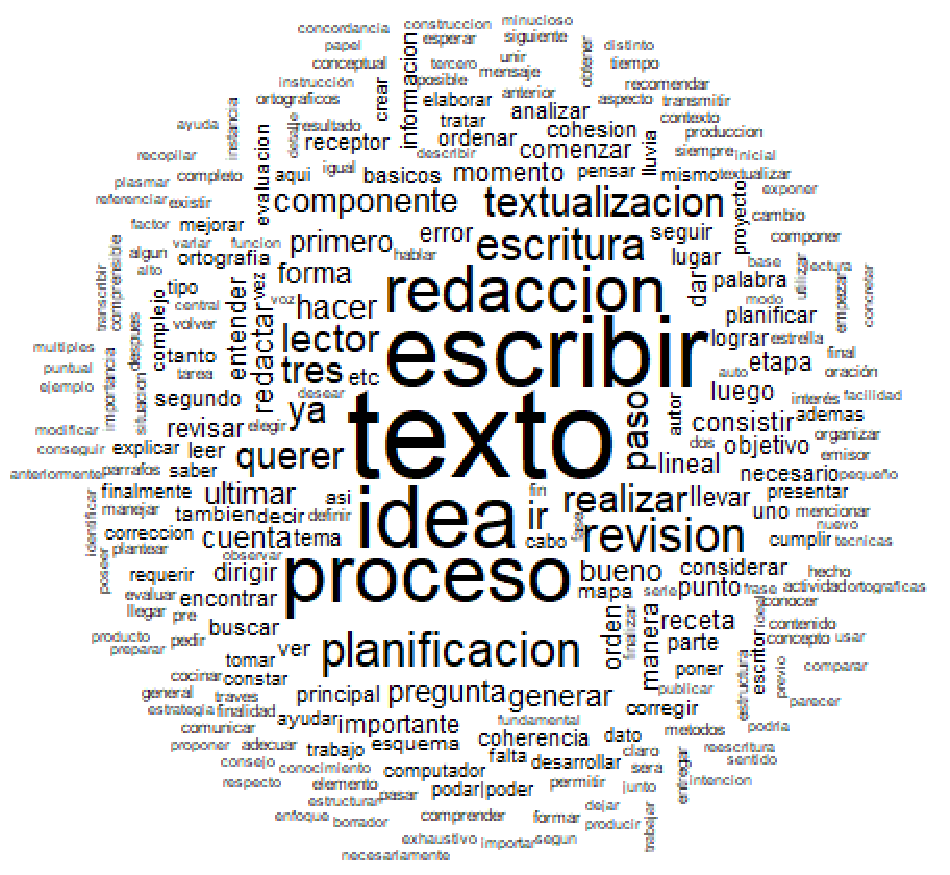
\includegraphics[width=\textwidth]{figure01}
\source{\cite{dmitrenko2020autonomous}.}
\end{minipage}
\end{figure}
The created e-textbook allowed the students to \begin{enumerate*}[label=\arabic*)]
	
	\item practice professional
	lexical skills; 
	\item carry out current control of the understanding of the
	content of the text on the specialty; 
	\item communicate using the learnt
	professional vocabulary; 
	\item discuss educational and professional problem
	situations; 
	\item prepare public speeches on a number of professional
	issues; 
	\item search for new textual, graphic and audio professionally
	oriented English information and analyze it; 
	\item write professional
        letters and documents in English (\Cref{fig-02}).
\end{enumerate*}

\begin{figure}[htpb]
\centering
\begin{minipage}{.65\textwidth}
\caption{Screenshot of the page (listening to the dialogue) of the e-textbook \enquote{Mathematics}.}	
\label{fig-02}
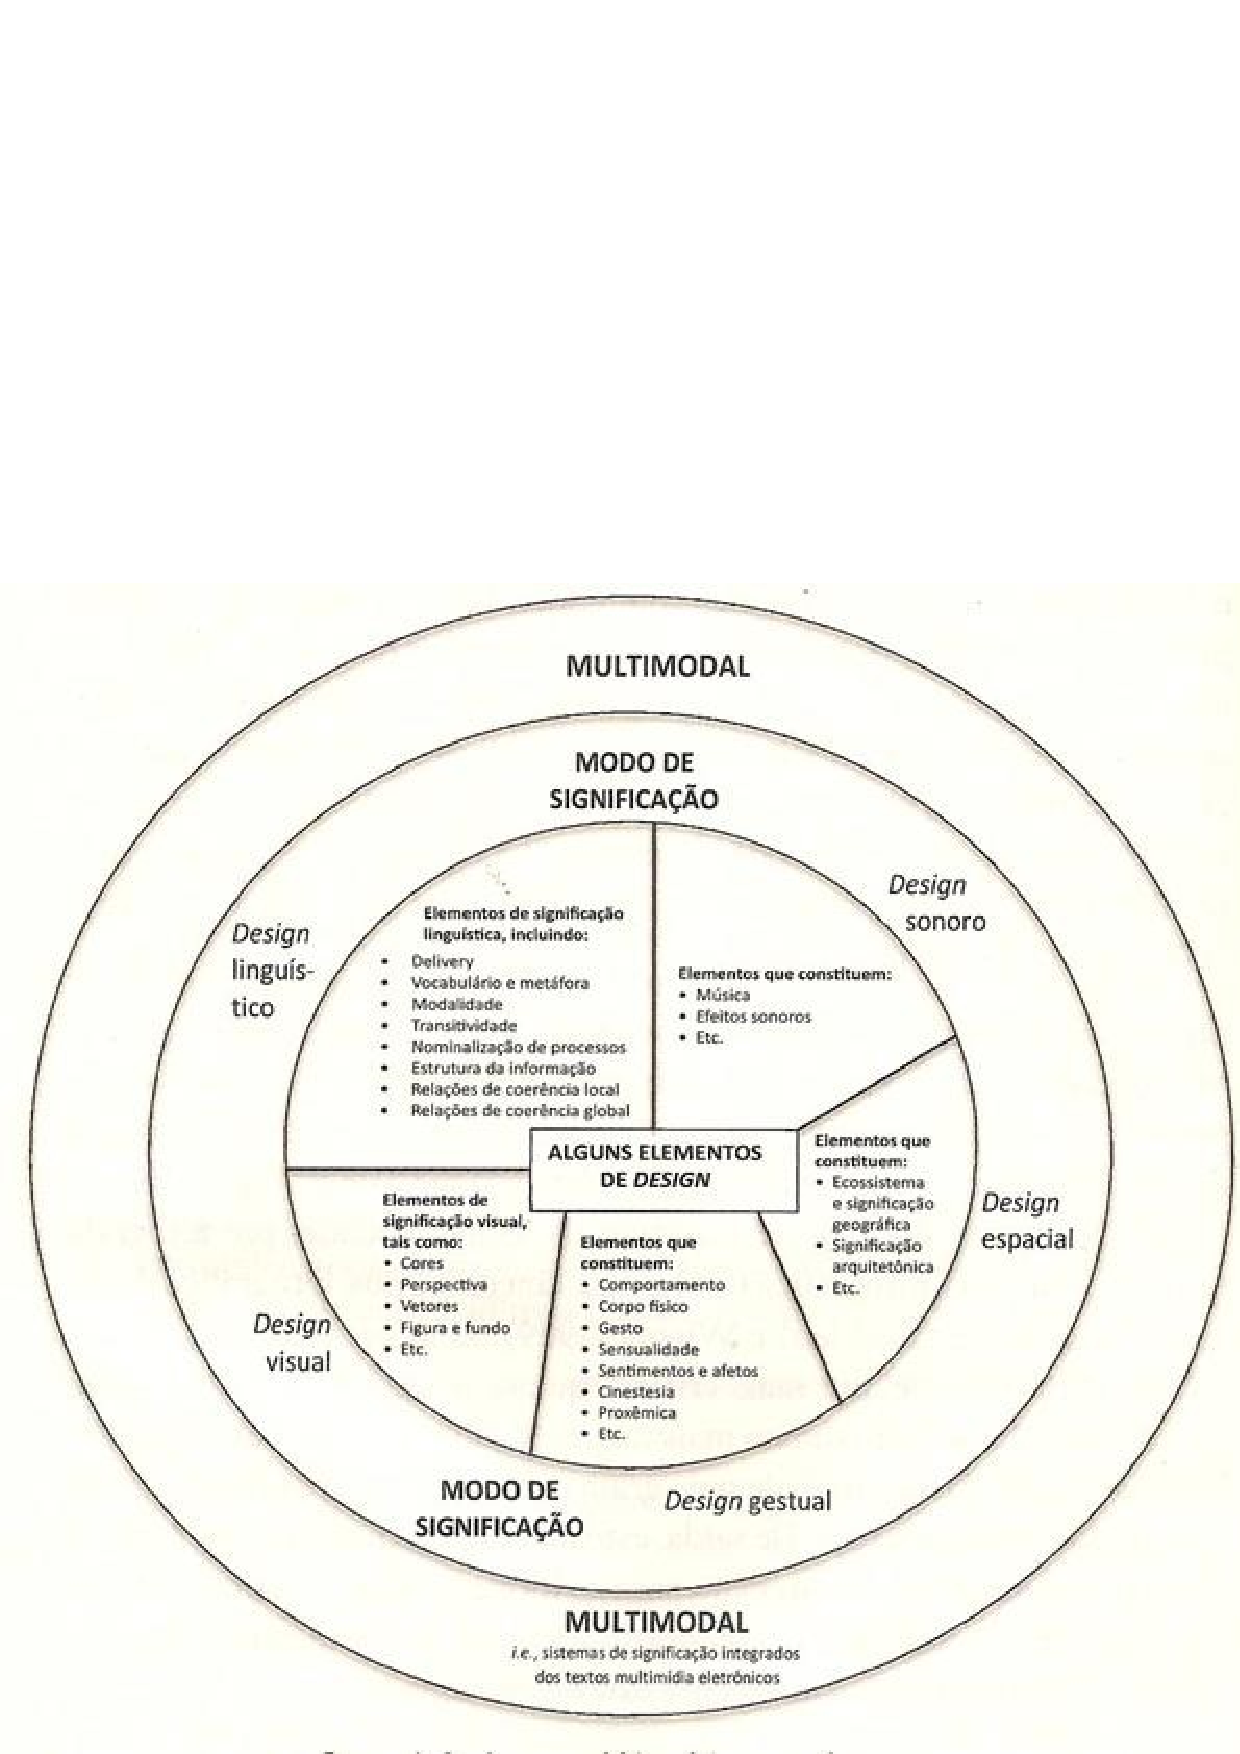
\includegraphics[width=\textwidth]{figure02}
\source{\cite{dmitrenko2020autonomous}.}
\end{minipage}
\end{figure}

Various applications have been used for interactive online ESP classes.
For example, the universal designer of interactive tasks
LearningApps.org was used to support the ESP learning process with the
help of interactive modules. Both the teacher and the student could
create interactive tasks based on ready-made templates. Such
verification and consolidation of the students' knowledge in a playful
way contributed to the formation of their cognitive interest in the ESP
educational component. The service included a gallery of publicly
available interactive tasks in English and all learning materials might
be posted publicly or for private use. An effective mobile web-based
learning application for ESP classes Quizlet was used to study and
repeat lexical and grammatical material with the help of self-made
flashcards, which contributed to the rapid assimilation of English
training material. The Quizlet Live application allowed students to
check the quality of the learned lexical material in an individual or
group format. The Kahoot!, was used to create tests, games, and quizzes
and is freely accessible from any browser on any device with internet
access. The teacher could create (or use a database of ready-made ones)
interactive tests, lead discussions, and present other learning
materials. Some examples of applications for creating exercises are
presented below.

\textbf{Example 1}. The purpose of the exercise is to acquaint students with the
typical features of using computers, to check the level of understanding
of the text, and to read silently (intensive reading). Instructions:
\enquote{Follow the link. Read the first paragraph of the text and write the
title. Check the correct answer by clicking on the button \enquote{Check
your answer}. Click on the arrow and move to another paragraph. You
have 15 minutes to do this} (\Cref{fig-03}).

\begin{figure}[htpb]
\centering
\begin{minipage}{.65\textwidth}
\caption{An example of an exercise in the application Learning Apps.}	
\label{fig-03}
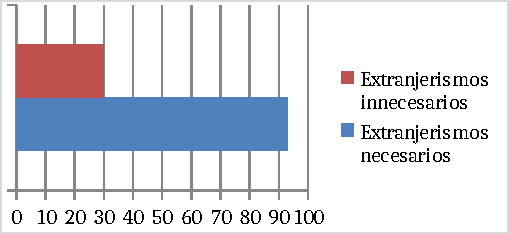
\includegraphics[width=\textwidth]{figure03}
\source{\cite{dmitrenko2020autonomous}.}
\end{minipage}
\end{figure}

\textbf{Example 2}. The exercise aims to check the level of understanding of
lexical items from the text. Instructions: \enquote{Follow the link. Match the
word with its definition. While doing the task, you will see the timer
which will count the time you have to complete the exercise. If you
choose the wrong answer, the time will be doubled. The person who
completes the task the fastest gets the highest score} (\Cref{fig-04}).

\begin{figure}[htpb]
\centering
\begin{minipage}{.65\textwidth}
\caption{A sample of an exercise in the Quizzlet application.}	
\label{fig-04}
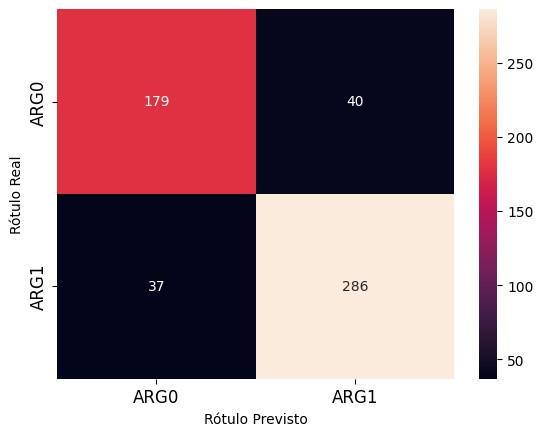
\includegraphics[width=\textwidth]{figure04}
\source{\cite{dmitrenko2020autonomous}.}
\end{minipage}
\end{figure}

\textbf{Example 3}. The purpose of the exercise is to check the level of reading
comprehension and text analysis. Instructions: \enquote{Take your mobile
phone and follow the link (\url{https://kahoot.it/}). Ask your teacher
for the code, enter it and your name. On the teacher's screen, you will
see the fact about computers and two sentences with red and blue colors.
Read the fact and choose the right color for yourself on the phone. If
you already know the fact, then you are doing great. If you don't know
the fact, then explain what exactly you want to discover about it. The
one who shares the opinion the most of all will get the highest score}
(\Cref{fig-05}).


\begin{figure}[htpb]
\centering
\begin{minipage}{.65\textwidth}
\caption{An example of an exercise in Kahoot!}	
\label{fig-05}
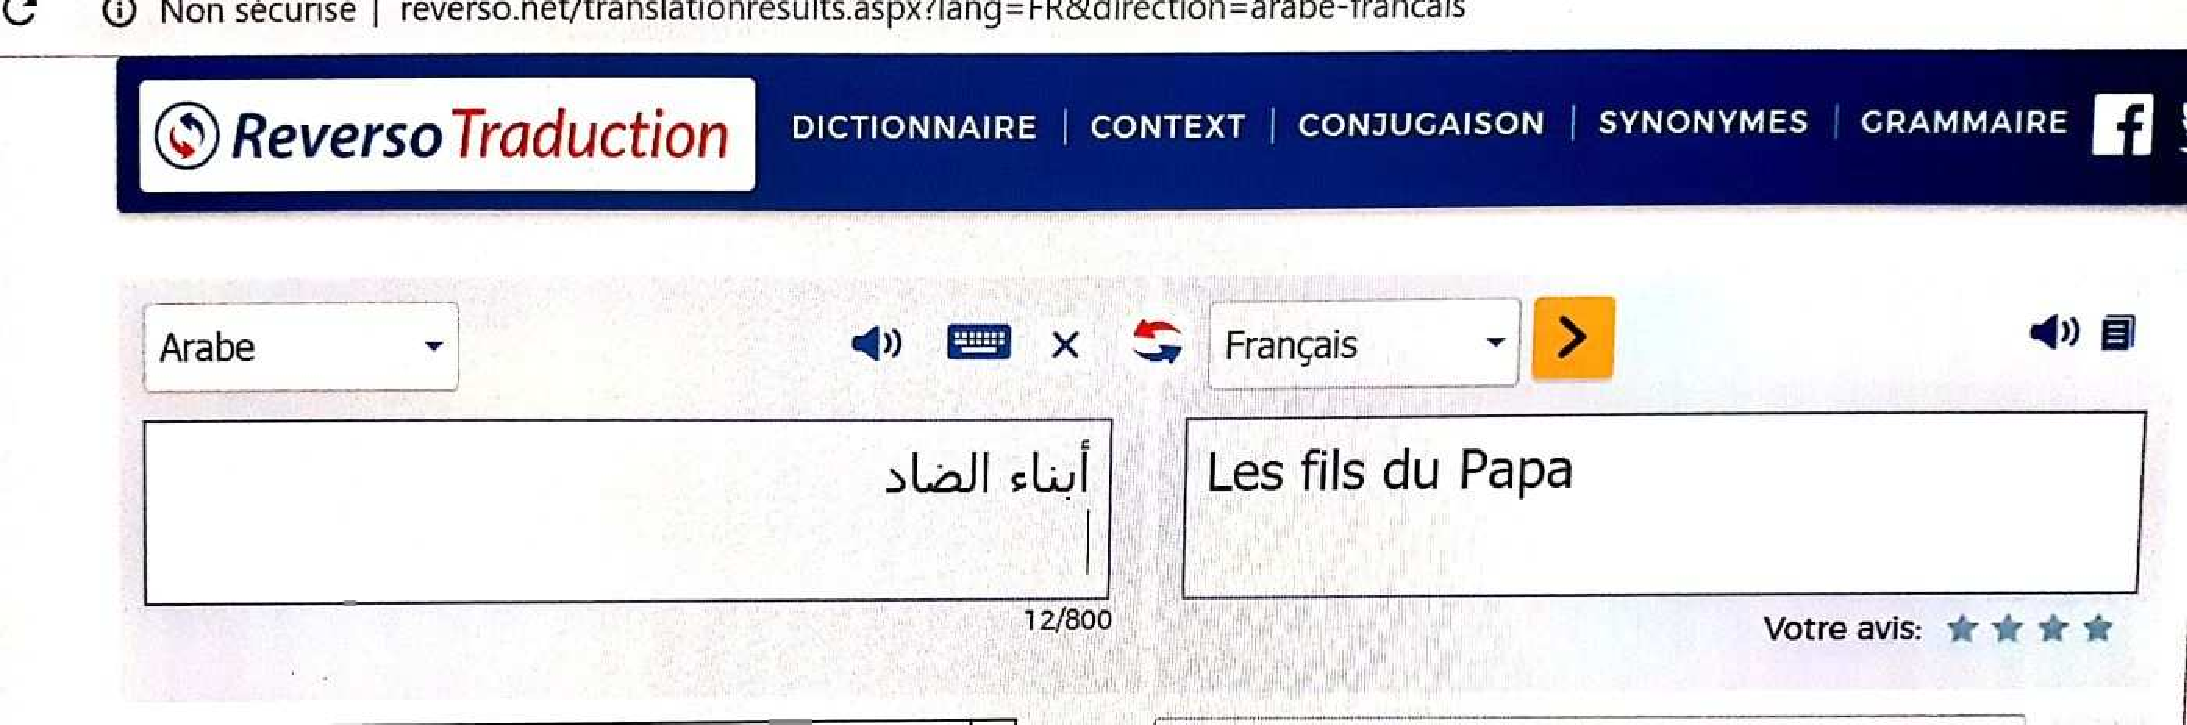
\includegraphics[width=\textwidth]{figure05}
\source{\cite{dmitrenko2020autonomous}.}
\end{minipage}
\end{figure}

\subsubsection{Participants}\label{subsubsec-participants}

The pre-service teachers of mathematics were divided into two
homogeneous groups: the control group (CG) – the formation of POACC
under usual conditions and the experimental group (EG) – the formation
of POACC under the influence of an active pedagogical factor – with the
use of virtual resources and digit tools. The participants of the study
were second-year students of the specialisation \enquote{Secondary Education.
Mathematics}, and \enquote{Mathematics} at the Faculty of Mathematics,
Physics and Computer Sciences, Vinnytsia Mykhailo Kotsiubynskyi State
Pedagogical University. The total number of participants was 100
students, 50 participants in CG and EG respectively. The experimental
training was carried out during one semester (17 weeks), and the ESP
classes were held twice a week. The ESP classes were held synchronously
online and lasted 80 minutes. Students were informed about the goals,
tasks, and conditions of experimental training and participated
voluntarily.

\subsubsection{The Study Stages}\label{subsubsec-thestudystages}

The study on the appropriateness of using ICT technology in ESP learning
by pre-service teachers of mathematics consisted of three stages. The
task of the \emph{first} stage was to measure the level of development
of the POECC of pre-service teachers of mathematics in EG and CG at the
beginning of the experimental training. The task of the \emph{second}
stage was to carry out the actual experimental training of ESP in EG
using the developed technology of ICT with virtual resources and digital
tools, and traditional training (without ICT tools) in CG. The task of
the \emph{third} stage was to diagnose and compare the level of
development of POECC of pre-service teachers of mathematics in CG and EG
after the introduction of an active pedagogical influence factor,
namely, the educational technology of using ICT in ESP learning.

\subsubsection{Instruments}\label{subsubsec-instruments}

The students' level of POECC was measured at the beginning and after the
experimental training (pre- and post-phases). The test was administered
to the students to assess the development of POECC according to the
following learning outcomes, which included 4 parts: \begin{enumerate*}[label=\arabic*)]
\item  knowledge of
basic English professional terms; 
\item the ability to translate
professional texts; 
\item the ability to analyze the content of English
professional sources; 
\item the ability to listen and understand the oral
professional speech.
\end{enumerate*}

The evaluation was carried out by experts (English teachers) on a
100-point scale for four components: knowledge of basic English
professional terms, translation of professional texts, content analysis
of English professional sources, and the ability to listen to oral
professional speech. Each component was evaluated in terms of 25 points.
The maximum level of development of each component was estimated at a
maximum of 25 points; the possible minimum was 1 point. The total score
for all components determined the level of development of the POECC of
pre-service teachers of mathematics: a low level – from 4 to 40 points;
an average level – from 41 to 74 points; and a high level – from 75 to
100 points. The assessment was carried out according to the
methodological recommendations of a group of experts.

The initial part of the test assessed the participants' understanding of
fundamental mathematical terms in English. The task required the
translation of fifty English terms, with each correct answer being
awarded two points. The second part of the test evaluated the students'
ability to translate professional English texts from English into
Ukrainian. Students were given to read and translate an English
professional text on a mathematical topic. The third part of the test
assessed students' capacity to analyze professional English sources and
select the appropriate section for further detailed study, analysis, and
use in pedagogical practice. The fourth part of the test evaluated
students' ability to comprehend spoken English in a professional
context. They were required to listen to a professional English text and
translate it into Ukrainian.

To assess group homogeneity and result reliability, we performed
statistical processing on the data using Pearson's $\chi^2$ test.
We calculated the empirical value using the formula:

\begin{equation}\label{eq-01}
X^{2}_{emp} = N . M . \sum_{i=1}^{L}\frac{ (\frac{n_{i}}{N}-\frac{m_{i}}{M})^{2}}{n_{i}+m_{i}}
\end{equation}
 
%{\begin{center}
%\large$X^{2}_{emp} = N . M . \sum_{i=1}^{L}\frac{ (\frac{n_{i}}{N}-\frac{m_{i}}{M})^{2}}{n_{i}+m_{i}} \label{formula-01}$
%\end{center}}

\begin{itemize}
    \item N and M represent the numbers of EG and CG members respectively.
    \item The i-th level of pre-service teachers' readiness for ESP online
learning was demonstrated by the number of EG and CG members.
    \item The variable L represents the quantity of chosen levels. 
    \item The data was processed using the Microsoft Excel 2019 program.
\end{itemize}

\section{Results}\label{sec-results}

This section is divided into three main topics. First, we will discuss
the social media platforms and languages students use, along with the
objectives they pursue when making videos. Second, we will describe what
students do before and after making videos. Third, we will examine
students' perceptions of language learning through video-making.

\subsection{Social media platforms, languages, and objectives}\label{sub-sec-socialmediaplatforms}

In general, 46 people, or only 21.7\% of the participants of the overall
questionnaire, reported that they occasionally had been making videos in
a broad sense (including reels and stories on Instagram). We will centre
most of our results section on these participants.

Stories on Instagram and videos on YouTube were the most frequently
produced types of videos according to \Cref{fig-01}. Instagram stories are
used 28.3\% \emph{sometimes} and 13\% \emph{frequently}, meanwhile,
videos on YouTube are made 34.8\% \emph{sometimes} and 8.7\%
\emph{frequently}. Notably, almost nobody used Twitch and a small
percentage of the students made videos on TikTok (15.2\%).

\begin{figure}[htbp]
\centering
\begin{minipage}{\textwidth}
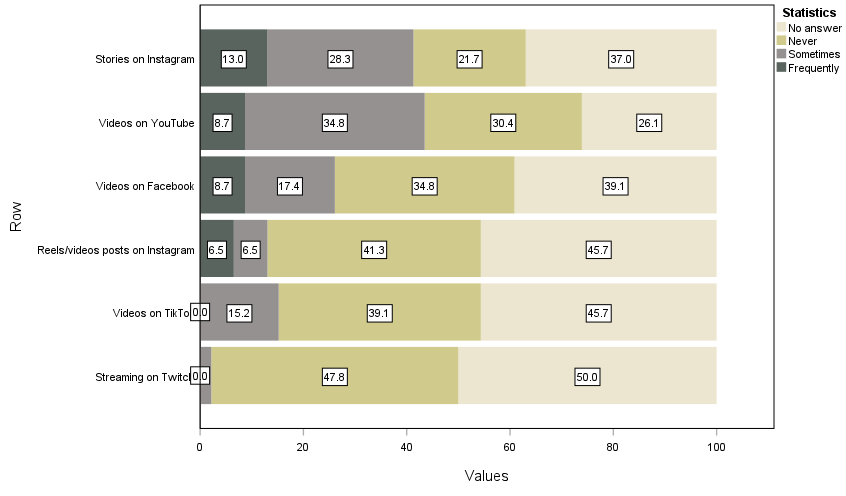
\includegraphics[width=\textwidth]{Fig-1.png}
\caption{Frequency of production of different types of videos.}
\label{fig-01}
\source{Own elaboration.}
\end{minipage}
\end{figure}

We also observe a pattern across all platforms, with the least common
response being to make videos frequently (from 13\% on Instagram to 0\%
on TikTok), indicating that a relatively low percentage of respondents
makes videos frequently, especially in comparison with the practice of
watching videos \cite{shafirova2023}. Moreover, we found a
correlation between the age of the students and the types of video
production. The correlation was found in the social media platforms of
TikTok, YouTube and Facebook, in which older students (older than 36)
tend to make videos for Facebook (due to cross tabulation with Pearson
chi-square test with 0.019 significance in case of YouTube and 0.004 in
case of Facebook). Meanwhile, younger students (from 18 to 23) tend to
make videos on TikTok (due to cross tabulation with Pearson chi-square
test with 0.008 significance). It is noteworthy that, on Instagram, we
did not find any correlation with age.

In general, in our data, age does not influence the frequency of making
videos, however, it points out that some social media platforms are more
frequently used by younger respondents and some by slightly older
respondents (similarly found in the dataset concerning the US population
from \textcite{ortizo-spina2019}). Moreover, the students post videos in
different languages, mostly in Portuguese and English (\Cref{tab-04}), while
other languages have a relatively smaller presence (max. 20\% with
Spanish on Facebook).

\begin{table}[htbp]
\centering
\begin{threeparttable}
\caption{Languages and platforms of video production: multiple choice response.}
\label{tab-04}
\begin{tabular}{*{11}{l}}
\toprule
Platforms & \multicolumn{2}{c}{YouTube} & \multicolumn{2}{c}{Facebook} &  \multicolumn{2}{c}{Instagram} & \multicolumn{2}{c}{TikTok} & \multicolumn{2}{c}{Twitch} \\
\midrule
Portuguese & 22 & 88\% & 13 & 86.7\% & 19 & 95\% & 5 & 71.4\% & 0 & 0\% \\
English    & 13 & 52\% & 6  & 40\%   & 9  & 45\% & 5 & 71.4\% & 1 & 50\% \\
Spanish    & 3  & 12\% & 3  & 20\%   & 1  & 5\%  & 0 & 0\%    & 0 & 0\% \\
Italian    & 2  & 8\%  & 2  & 13.3\% & 1  & 5\%  & 0 & 0\%    & 0 & 0\% \\
French     & 1  & 4\%  & 2  & 13.3\% & 0  & 0\%  & 0 & 0\%    & 0 & 0\% \\
Crioulo    & 0  & 0\%  & 0  & 0\%    & 1  & 5\%  & 0 & 0\%    & 0 & 0\% \\
Persian    & 0  & 0\%  & 1  & 6.7\%  & 0  & 0\%  & 0 & 0\%    & 0 & 0\% \\
Other      & 2  & 8\%  & 1  & 6.7\%  & 1  & 5\%  & 2 & 28.6\% & 1 & 50\% \\
\rule{0pt}{3ex}%
Total & 44 & 176\% & 28 & 186.7\% & 32 & 160\% & 12 & 171.4\% & 2 & 100\% \\
\bottomrule
\end{tabular}
\source{Own elaboration.}
\end{threeparttable}
\end{table}




In comparison, our previous study shows that video consumption on social
media and streaming platforms could be considered more diverse and
plurilingual. Even though English and Portuguese were still the most
popular languages, Spanish was used by roughly half of the participants
on streaming platforms such as Netflix and HBO. Additionally, such
languages as French, Italian, Korean or Japanese were also present, with
more than 10\% on various platforms \cite{shafirova2023}. There
could be various reasons for this difference in language variety in
video production and consumption. One possible explanation could be the
amount of resources available for watching videos in languages you do
not have a perfect command of, such as subtitles in different languages,
captions, scripts and more \cite{shafirova2023}.

Moreover, we asked the participants if they tended to use several
languages in one video. The participants responded with 26.1\% ``yes'',
with the main objective of reaching out to a vast audience (41.6\%), or
because of being multilingual (30\%).

\subsection{Why students make and post videos}

To understand students' intentions behind video production, we asked
about their objectives when making videos. According to \Cref{fig-02}, the
majority of the students make videos to ``have fun'' (63\%), which goes
along with previous research on video creation beyond the classroom
\cite{zhang2022}.

\begin{figure}[htbp]
\centering
\begin{minipage}{\textwidth}
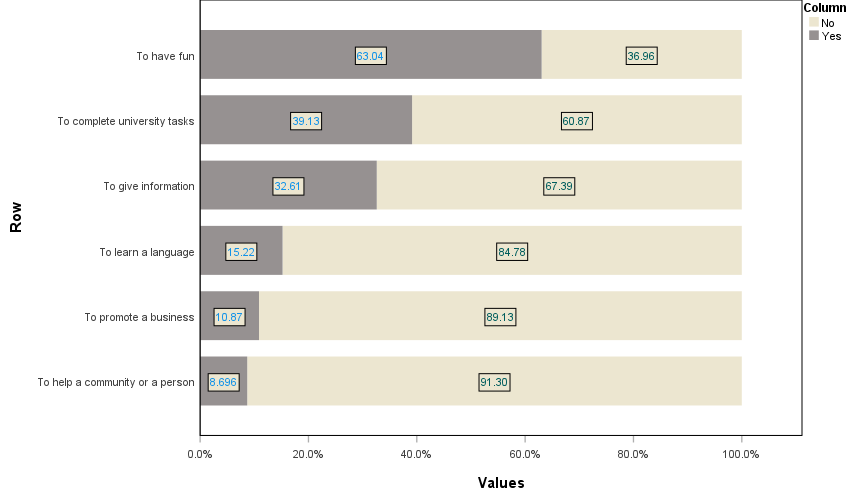
\includegraphics[width=\textwidth]{Fig-2.png}
\source{Own elaboration.}
\caption{Objectives to make videos.}
\label{fig-02}
\end{minipage}
\end{figure}

However, the second most popular answer is ``to complete university
tasks'' (39.1\%), which is a thought-provoking result indicating that
some of the university tasks require students to make videos (similar
results at the school level in \textcite{cassany2021}). It would be
valuable to explore the potential differences between the videos created
for leisure and those made as university tasks, even though these videos
would not necessarily be connected to language learning.

Moreover, the third answer was ``to give information'' (33\%), which
also seems like a serious and not entertaining goal, which can include
making videos or reposts of some news or events. This goes against the
assumption of some researchers that social media is always used only for
entertainment purposes \textcite{rosyida2019}. Also, the option ``to
learn a language'' was not popular (15.2\%), which is an expected result
as only 33\% of the participants are current language learners.

\subsection{What students do before and after producing videos}

Much like when watching videos online \cite{shafirova2023},
around half of the respondents were engaged in some communicative
actions before and after making a video. According to \Cref{tab-05} and \Cref{tab-06},
the communicative actions included searching (information or visuals),
reading (comments), writing (descriptions of the videos), watching
videos (to analyse similar videos), translating and interacting with
others (collaborating with others, responding to comments, making video
responses). The most frequent action before video production is
searching for information (\Cref{tab-05}), while the most frequent after
production is reading the comments or feedback on the videos (\Cref{tab-06}).
The options of writing descriptions or interacting with others were less
popular (roughly half of the responses).


\begin{table}[htbp]
\centering
\small
\begin{threeparttable}
\caption{Communicative actions made before video production.}
\label{tab-05}
\begin{tabular}{*{13}{l}}
\toprule
\multicolumn{1}{{>{\raggedright\arraybackslash}p{0.11\textwidth}}}{Actions} &
\multicolumn{2}{{>{\raggedright\arraybackslash}p{0.11\textwidth}}}{Search for information} &
\multicolumn{2}{{>{\raggedright\arraybackslash}p{0.11\textwidth}}}{Search for visual aid} &
\multicolumn{2}{{>{\raggedright\arraybackslash}p{0.11\textwidth}}}{Analyse similar videos} &
\multicolumn{2}{{>{\raggedright\arraybackslash}p{0.11\textwidth}}}{Write short descriptions} &
\multicolumn{2}{{>{\raggedright\arraybackslash}p{0.11\textwidth}}}{Collaborate with others} &
\multicolumn{2}{{>{\raggedright\arraybackslash}p{0.11\textwidth}}}{Make translations} \\
\midrule
Languages & N & \% & N & \% & N & \% & N & \% & N & \% & N & \% \\ 
Portuguese & 16 & 69.6\% & 11 & 47.8\% & 10 & 43.5\% & 11 & 47.8\% & 9  & 39.1\% & 7  & 30.4\% \\ 
English    & 18 & 78.3\% & 15 & 65.2\% & 11 & 47.8\% & 7  & 30.4\% & 7  & 30.4\% & 9  & 39.1\% \\ 
Spanish    & 3  & 13\%   & 2  & 8.7\%  & 3  & 13\%   & 1  & 4.3\%  & 2  & 8.7\%  & 1  & 4.3\%  \\ 
Italian    & 2  & 8.7\%  & 2  & 8.7\%  & 2  & 8.7\%  & 1  & 4.3\%  & 2  & 8.7\%  & 1  & 4.3\%  \\ 
French     & 2  & 8.7\%  & 2  & 8.7\%  & 2  & 8.7\%  & 0  & 0\%    & 2  & 8.7\%  & 1  & 4.3\%  \\ 
Chinese    & 1  & 4.3\%  & 1  & 4.3\%  & 0  & 0\%    & 1  & 4.3\%  & 0  & 0\%    & 0  & 0\%    \\ 
Persian    & 1  & 4.3\%  & 0  & 0\%    & 0  & 0\%    & 0  & 0\%    & 0  & 0\%    & 0  & 0\%    \\ 
Other      & 1  & 4.3\%  & 0  & 0\%    & 0  & 0\%    & 0  & 0\%    & 0  & 0\%    & 0  & 0\%    \\ 
\rule{0pt}{3ex}%
Total     & 44 & 191.2\% & 33 & 143.4\% & 28 & 121.7\% & 21 & 91.1\% & 22 & 95.6\% & 19 & 82.4\% \\ 
\bottomrule
\end{tabular}
\source{Own elaboration.}
\end{threeparttable}
\end{table}

Interestingly, if videos were mostly created in Portuguese and English,
the actions made before and after video production had more linguistic
variability, with the 7 languages present before video production, and
11 after production.

Furthermore, we made a comparison or cross-tabulation comparing the
participants\textquotesingle{} mother tongues with the actions taken
before video production (\Cref{tab-05}). The results showed that most
participants were using a foreign language before and after making a
video. In the case of activities made before video production, several
participants used such foreign languages as English, French and Italian.
Also, some participants used their mother tongues, including Portuguese,
Spanish, Chinese and Persian. Similar data emerged when comparing the
responses concerning the actions taken after posting the videos in
relation to the participants' mother tongues (\Cref{tab-06}).


\begin{table}[htbp]
\centering
\begin{threeparttable}
\caption{Communicative actions made after video production.}
\label{tab-06}
\begin{tabular}{*{7}{l}}
\toprule
Actions &
\multicolumn{2}{{{>{\raggedright\arraybackslash}p{0.25\textwidth}}}}{Read comments, chat, reactions} &
\multicolumn{2}{{>{\raggedright\arraybackslash}p{0.14285714285\textwidth}}}{Respond to the comments} &
\multicolumn{2}{{>{\raggedright\arraybackslash}p{0.14285714285\textwidth}}}{Make video responses to comments} \\
\midrule
Portuguese & 19 & 79.2\% & 8 & 33.3\% & 3 & 12.5\% \\ 
English    & 17 & 70.8\% & 9 & 37.5\% & 3 & 12.5\% \\ 
Spanish    & 7  & 29.2\% & 3 & 12.5\% & 1 & 4.2\%  \\ 
Italian    & 5  & 20.8\% & 3 & 12.5\% & 1 & 4.2\%  \\ 
French     & 5  & 20.8\% & 2 & 8.3\%  & 2 & 8.3\%  \\ 
Chinese    & 2  & 8.3\%  & 1 & 4.2\%  & 1 & 4.2\%  \\ 
Persian    & 2  & 8.3\%  & 1 & 4.2\%  & 2 & 8.3\%  \\ 
Russian    & 2  & 8.3\%  & 1 & 4.2\%  & 1 & 4.2\%  \\ 
Korean     & 1  & 4.2\%  & 1 & 4.2\%  & 1 & 4.2\%  \\ 
Crioulo    & 1  & 4.2\%  & 1 & 4.2\%  & 1 & 4.2\%  \\ 
Japanese   & 1  & 4.2\%  & 1 & 4.2\%  & 1 & 4.2\%  \\ 
Other      & 1  & 4.2\%  & 1 & 4.2\%  & 2 & 8.3\%  \\ 
Total      & 63 & 262.5\% & 32 & 133.5\% & 19 & 79.3\% \\ 
\bottomrule
\end{tabular}
\source{Own elaboration.}
\end{threeparttable}
\end{table}

For instance, in \Cref{tab-06}, most participants used English as a foreign
language when reading and responding to comments. Other foreign
languages included Spanish (only one respondent used it as a mother
tongue), French, Italian and Korean. These data indicate that students
engaged in communicative activities in foreign languages both before and
after making a video. This characterizes video production as interactive
and increases language input through various modes, including written,
oral, interactive, and information-seeking activities.

\subsection{The students' perceptions of language learning with video production and consumption}

The questionnaire included two questions about students' perceptions of
language learning while watching or producing videos. The questions went
as follows: ``To what extent do you agree with the statement:
Watching/producing videos in (an)other language(s) helped me in learning
this(ese) language(s)''.

In \Cref{fig-03}, we compare the answers to these questions divided into two
graphics (based on N-46), one focused on video viewing (blue) and the
other on video production (red). The line on video viewing is much more
accentuated in comparison with video production which has an almost
normal distribution.

\begin{figure}[htbp]
\centering
\begin{minipage}{\textwidth}
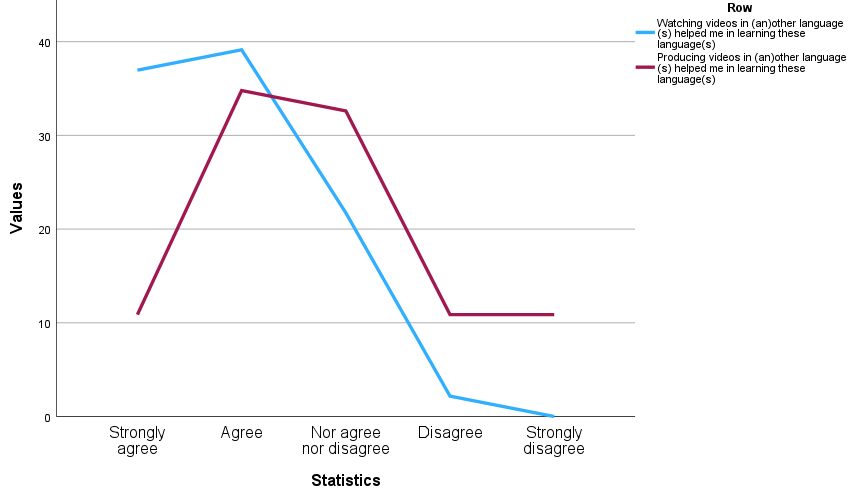
\includegraphics[width=\textwidth]{Fig-3.png}
\caption{Students' perceptions of language learning with the help
	of video watching/producing.}
\label{fig-03}
\source{Own elaboration.}
\end{minipage}
\end{figure}

It indicates that in the case of video watching, the students mostly
``strongly agree'' and ``agree'' (around 75\%) with the proposed
statement. However, in the case of video producing, most respondents
``agree'' or ``neither agree nor disagree'' (around 70\%), with some
respondents ``disagreeing'' and ``strongly disagreeing'' (around 22\%).
This comparison shows a division in opinions on the benefits of video
production, with more uncertainty in the results for video production
compared with video watching.

These results could be connected to the frequency of video production
compared to video viewing and the fact that students could be engaged in
very different forms of video production, from Instagram stories to
lengthy videos on YouTube. It can also be connected to our particular
dataset which includes students from non-language studies. In general,
we consider this discrepancy in data on video viewing and production an
interesting phenomenon for further investigation.

Additionally, we ran a cross-tabulation test with a Pearson Chi-Square
test to examine if there is a correlation between these students'
perceptions of video production (\Cref{fig-03}) and the fact that they are
current language learners (\Cref{tab-03}). The p-value (or significance) for
the Chi-Square test was 0.6, indicating no significant correlation
between these two variables. However, due to the small sample size,
seven cells had an expected count of less than 5, which may make the
results unreliable. To address this, we combined the cells ``agree'' and
``strongly agree,'' as well as ``disagree'' and ``strongly disagree,''
transforming the 5-level Likert scale into a 3-level scale. In this
adjusted analysis, only two cells had an expected count of less than 5,
making the results more reliable. Similar to the previous test, the
p-value was 0.3, indicating no significant correlation between these
categories. In addition, we ran the Fisher Exact test which is better
suited for smaller samples, nevertheless, it also did not indicate any
correlation ($p=0.7$ in the first case and $p=9.4$ in the second case).

These results indicate that there is no significant correlation between
these two categories. We also examined the categories of current
language learners and students\textquotesingle{} perceptions of video
watching, and similarly found no correlation (Chi-Square test, $p=0.5$;
Fisher Exact test, $p=0.7$). However, it would be beneficial to test this
hypothesis with a larger dataset to confirm these findings.

Moreover, we examined the relationship between the category of students'
perceptions of video production benefits and the departments where the
students study. We combined our categories into 1) Language Department,
2) Education and Psychology, and 3) Other to see if there are some
correlations between our specific dataset and the question. The
Chi-Square test showed no significant correlation $(p= 0.066)$, however,
the Fisher Exact test showed some significance $(p = 0.05)$. In this case,
as our dataset is small and 50\% of the results have an expected count
of less than 5, the Fisher Exact Test seems to be more reliable \cite{jung2014}.
\Cref{fig-04} also shows a strong indication of dependence between
these categories.

\begin{figure}[htbp]
\centering
\begin{minipage}{\textwidth}
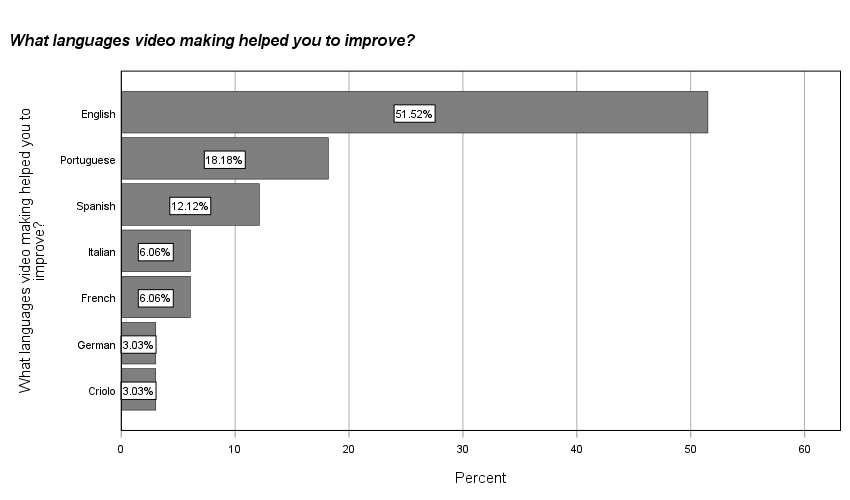
\includegraphics[width=\textwidth]{Fig-4.png}
\caption{Perceptions of the students on video production:
	department distribution.}
\label{fig-04}
\source{Own elaboration.}
\end{minipage}
\end{figure}

According to \Cref{fig-04}, we can see that in the Languages and Cultures
department, most students agree that video production helps in learning
a language (adjusted residual 1.6), while in Other Departments fewer
people agree with this statement (adjusted residual -2.5). In the
Department of Education and Psychology, fewer students disagreed that
video production could help language learning (adjusted residual -1.8).
The distribution observed here indicates more positive perceptions of
video production in the Department of Languages and Cultures. This
suggests that teaching methodologies in the Languages and Cultures and
the Education and Psychology departments may be influencing
students\textquotesingle{} perceptions. Additionally, when we tested the
correlation between a departmental distribution and students'
perceptions of video watching, we found no significant correlation using
either the Chi-Square test $(p=0.3)$ or the Fisher Exact test $(p=0.3)$.
Examining this question across different departments would be
beneficial, as our current dataset is too small to draw definitive
conclusions.

Moreover, 46\% of students chose the categories ``strongly agree'' and
``agree'' with the benefits of video production for language learning.
They also answered the next question regarding the languages that
video-making helped them learn (\Cref{tab-05}).

\begin{figure}[htbp]
\centering
\begin{minipage}{\textwidth}
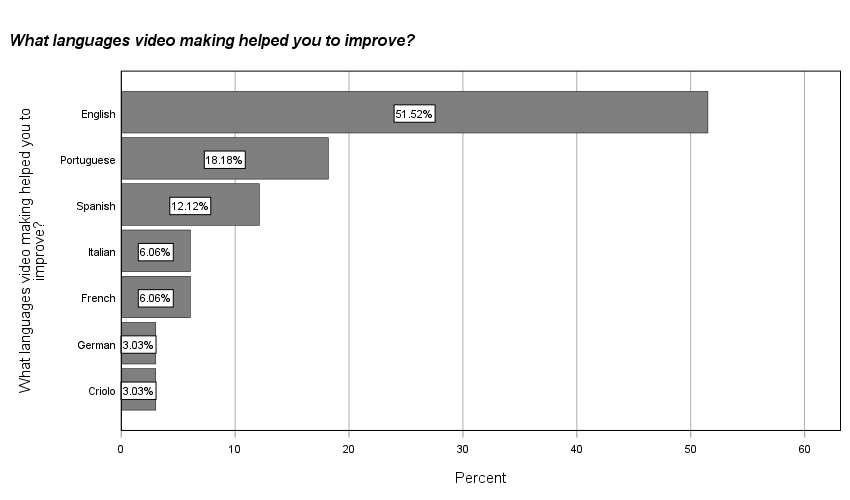
\includegraphics[width=\textwidth]{Fig-5.png}
\caption{Languages improved by making videos}
\label{fig-05}
\source{Own elaboration.}
\end{minipage}
\end{figure}

According to \Cref{fig-05}, the respondents chose a considerable variety of
languages, taking into account that only 21 people (from 46) responded
to that question and chose seven languages. English was the most popular
response, followed by Portuguese and Spanish. Notably, we can also see
\emph{Crioulo} derived from the Portuguese language (variation from Cabo
Verde) in the responses, which was completely absent from video viewing
responses \cite{shafirova2023}.

The students also responded to an open question concerning language
learning and video viewing/production: ``How have you improved your
language and cultural skills by watching/producing videos in different
languages?'' In the case of video viewing, we received 52 responses or
around 25\% of 212 respondents. According to our codebook (\Cref{annex-a}), 23
responses included the learning of vocabulary, oral comprehension had 9
responses, and pronunciation had 7. Students also noticed learning the
cultural aspects (7) of countries where languages are used and
underlined the importance of learning the language in the context of its
use (5). Overall, the detailed responses indicate that students view
this knowledge as important to share.

In the case of video production, we received 8 responses out of 46, in
other words, 17\% of the students responded, including such categories
as vocabulary (4), speaking (2) and cultural aspects (1). The answers
were less detailed than those in the viewing section, with a lower
overall response rate. Additionally, most responses came from the
Departments of Languages and Cultures and Education and Psychology. Some
responses highlighted that not only video production was beneficial for
language learning but also the work completed beforehand or afterwards
(\Cref{annex-a}). For instance, one respondent noticed: ``The research required
to produce most of my content has allowed me to widen my vision of the
English language and culture''.

We observe that students frequently highlighted vocabulary as the
primary area of improvement in both video viewing and production. This
suggests that, from the respondents\textquotesingle{} perspective,
vocabulary could be the most beneficial aspect of both practices.

\section{Conclusión}\label{sec-conclusión}

Las redes comunicativas sNOOC constituidas desde la formación de
posgrado y formadas por estudiantes que pasan a ser \emph{e-teacher} son
un ejemplo más de esfuerzo por la educación mediática inclusiva, en este
caso concreto, de la tercera edad. Gracias a plataformas como la de la
UNED, tmooc.es y el modelo sNOOC, se ha conseguido incentivar un modelo
formativo que pone de manifiesto un acceso equitativo y una
participación en la construcción colectiva del conocimiento. Esta
propuesta innovadora ha ayudado a consolidar un enfoque educativo y
comunicativo inclusivo adaptado a sectores vulnerables, a pesar de las
limitaciones del estudio como el tamaño de la muestra y la concreción de
los resultados en un contexto universitario determinado. La valoración
positiva de la experiencia formativa que hemos prestado en este artículo
no sólo destaca por su planteamiento didáctico o por la interacción de
las redes comunicativas creadas, sino que subraya el papel central de la
alfabetización mediática en la inclusión social de personas de la
tercera edad.

Es clave, como perspectiva futura, seguir fomentando la creación y
posterior investigación de redes comunicativas sNOOC, que asienten sus
proyectos formativos en acciones colaborativas y solidarias, potenciando
el uso de la inteligencia artificial, la gamificación y los entornos
inmersivos integrados en una pedagogía inclusiva. En un momento clave
para la formación a distancia, el reto de los agentes educativos y
sociales que se unen en red será mantener y mejorar la calidad del
modelo comunicativo y pedagógico, asegurando unas plataformas de
calidad, accesibles, adaptables y centradas en una comunicación
horizontal y bidireccional.

\printbibliography\label{sec-bib}
%conceptualization,datacuration,formalanalysis,funding,investigation,methodology,projadm,resources,software,supervision,validation,visualization,writing,review
\begin{contributors}[sec-contributors]
\authorcontribution{Pablo Ramírez Rodríguez}[conceptualization,datacuration,writing,investigation,resources,review,supervision,validation]
\authorcontribution{Evgeniy Antonov}[formalanalysis,datacuration,writing,methodology,resources,supervision,visualization]
\end{contributors}
\end{document}
